\subsection{BPNMs}
BPMN notation was used to ensure a thorough understanding and design of the key business processes taking place within the system. It enables a clear visual representation of task flows and interactions between the user, the system and the database \cite{white2004introduction}. Only chosen processes are described in this section. The selected processes were chosen based on their complexity and importance for the system: creating a new organisation, generating a production report, and creating a new must batch. Each diagram is divided into swimlanes that separate the actions of the actor from the application logic and, where relevant, from database operations. Gateways show validation and error paths, so that both the successful scenario and the cases in which the operation cannot be completed are documented.

The first two processes are presented together in Figure~\ref{fig:bpnm_organization} and Figure~\ref{fig:bpnm_reports}. Creating an organisation is the step that turns a newly registered account into a working vineyard in the system. Generating a report is the main analytical tool of the owner and involves searching production data, building a file and delivering it by e-mail. The third process, shown in Figure~\ref{fig:bpnm_must_batch}, is a representative production workflow of the oenologist: it combines form validation, a confirmation dialogue, a stock check and persistence of the new batch.

\begin{figure}[H]
    \centering
    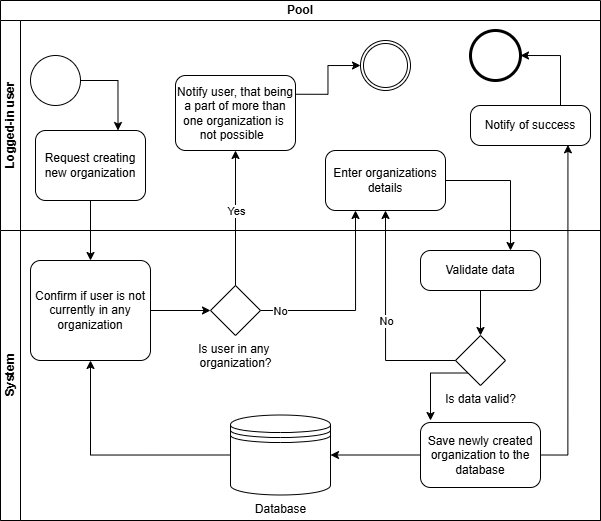
\includegraphics[width=0.92\textwidth,height=0.38\textheight,keepaspectratio]{pictures/create_organization_bpnm.drawio.png}
    \caption{A BPNM diagram presenting process of creating a new organization.}
    \label{fig:bpnm_organization}
\end{figure}
\begin{figure}[H]
    \centering
    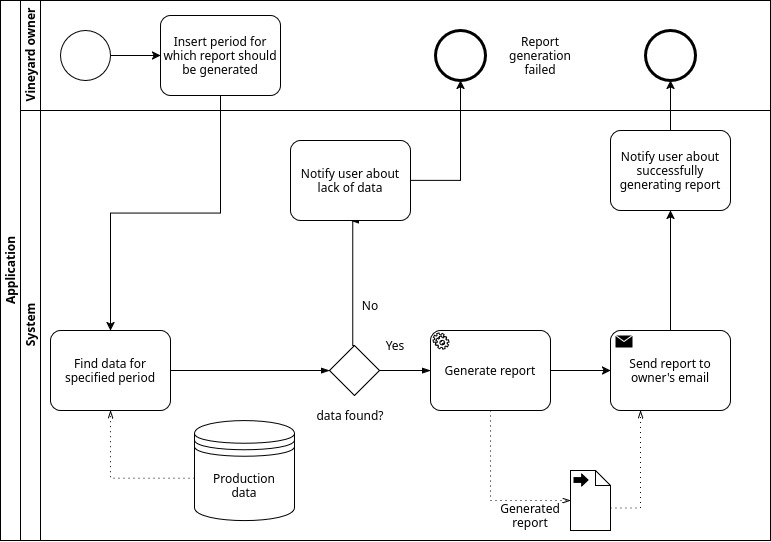
\includegraphics[width=0.92\textwidth,height=0.38\textheight,keepaspectratio]{pictures/generate_report_bpnm.jpg}
    \caption{A BPNM diagram presenting process of generating a report.}
    \label{fig:bpnm_reports}
\end{figure}

Figure~\ref{fig:bpnm_organization} starts when a logged-in user requests the creation of a new organisation. The application first loads user data from the database and checks whether that user already belongs to an organisation. Membership in more than one organisation is not allowed: if the check fails, the user is notified and the process ends. Otherwise the user enters organisation details, which the application validates. Invalid input returns the user to the form. When the data are valid, the new organisation is stored in the database and a success notification is shown.

Figure~\ref{fig:bpnm_reports} describes report generation from the vineyard owner's perspective. The owner provides the time period for which the report should be produced. The application searches production data for that period. If nothing is found, the owner is informed about the lack of data and the process ends with a failed generation. If records exist, the application generates the report file, sends it to the owner's e-mail address and notifies the user that generation has succeeded.

Figure~\ref{fig:bpnm_must_batch} presents the creation of a new must batch by the oenologist. After entering the batch data, the application checks whether the requested quantity exceeds the quantity of the selected fruit batch. If it does, an error is shown and the oenologist can correct the form. When the quantity is acceptable, a confirmation pop-up is displayed. Cancelling the dialogue returns the user to the form. After confirmation the system checks that the fruit is still in stock. Missing stock again results in an error notification. If stock is available, the must batch is created, the information is saved in the database, and the oenologist is notified that the operation succeeded.

\begin{figure}[H]
	\centering
	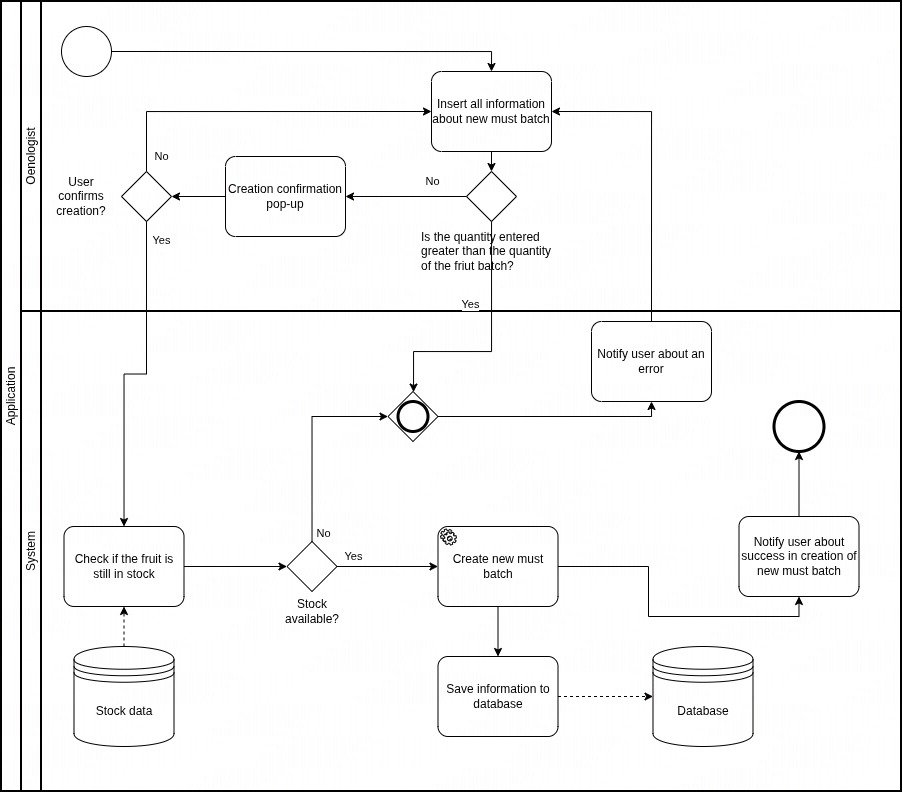
\includegraphics[width=0.92\textwidth,height=0.52\textheight,keepaspectratio]{pictures/create_new_must_batch_BPNM.jpg}
	\caption{A BPNM diagram presenting process of creating new must batch.}
	\label{fig:bpnm_must_batch}
\end{figure}

Together, the three diagrams cover onboarding of an organisation, reporting based on historical production data, and a typical batch-creation path in the winery. The same pattern of validation, confirmation and persistence appears in the remaining production stages (fermenting must, aged wine, blended wine and bottling), which is why those processes were not duplicated as separate BPMN models.
